\cohead{\Large\textbf{Sinus-/Cosinusfunktion}}
\fakesubsection{Definition der Sinus- und Cosinusfunktion}
Wie beim Bogenmaß beginnen wir beim Punkt \(P(1\vert 0)\) mit dem Bogenmaß \(b=0\) bzw. \(\alpha=0^\circ\) im Gradmaß.

\begin{minipage}{\textwidth}
	\adjustbox{valign=t}{\begin{minipage}{.257\textwidth}
		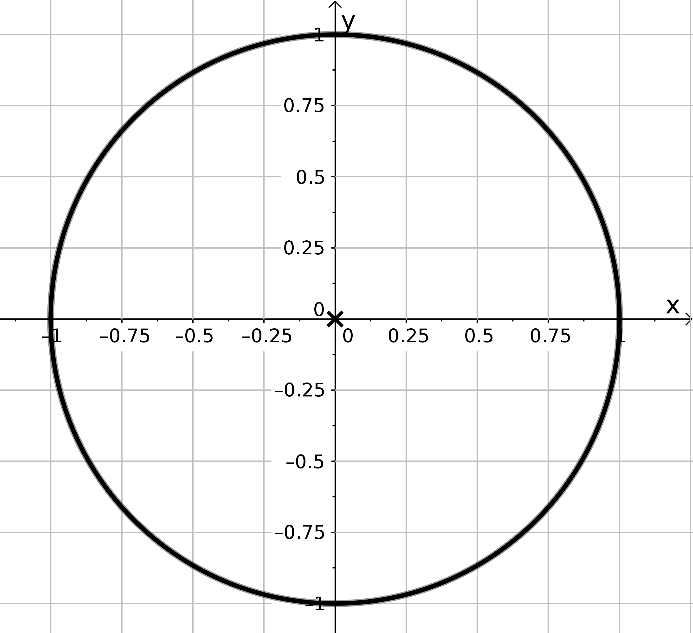
\includegraphics[width=\textwidth]{\trigonometrie/pics/Einheitskreis.png}
	\end{minipage}}%
	\adjustbox{valign=t}{\begin{minipage}{.743\textwidth}
		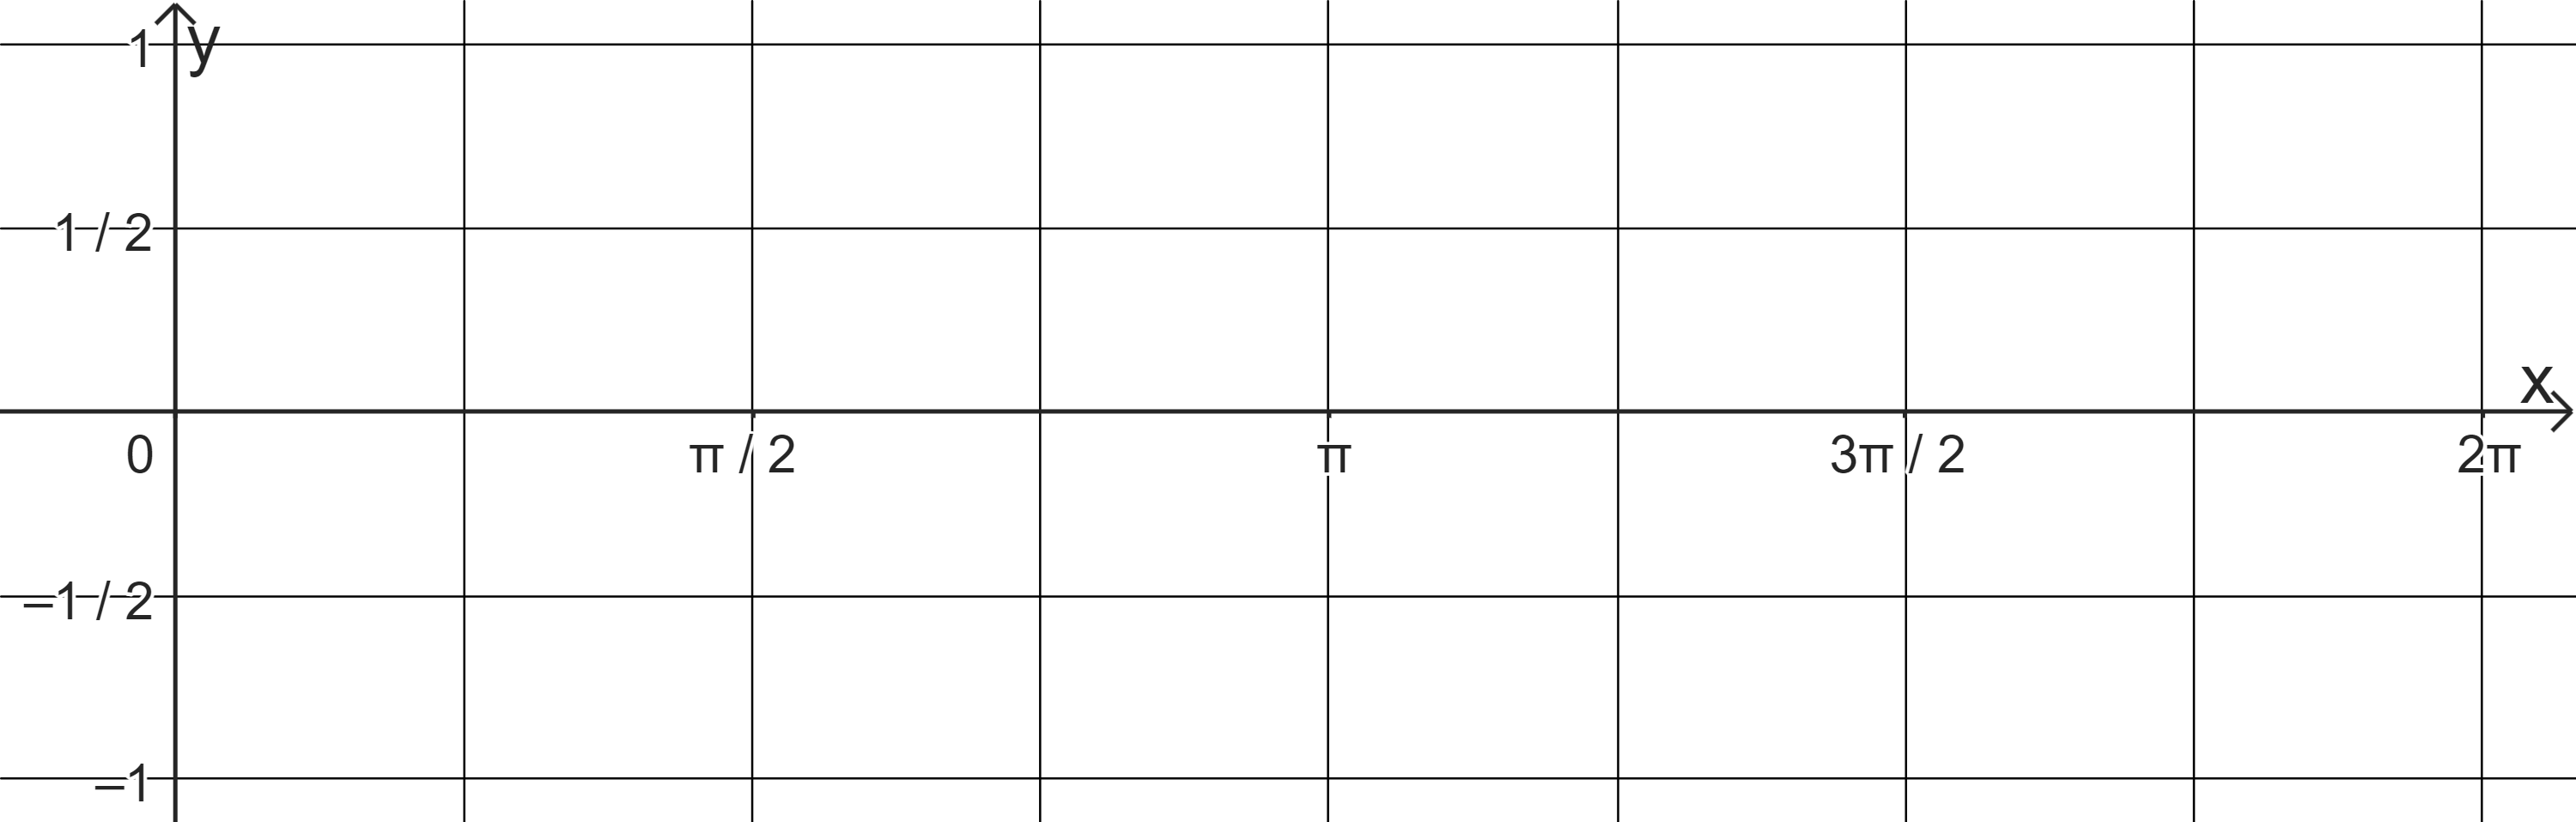
\includegraphics[width=\textwidth]{\trigonometrie/pics/leeresKoordinatensystem.png}
	\end{minipage}}%
\end{minipage}

\begin{tcolorbox}
	\textbf{Definition der Sinusfunktion}

	\textcolor{loestc}{Zu jedem Winkel \(b\) kann man genau einen Punkt \(P(x\vert y)\) auf dem Einheitskreis zuordnen. Der Sinus von \(b\) ist dann die \(y\)-Koordinate dieses Punkts:
		\[\sin\left(b\right)=y\]
	}
\end{tcolorbox}
Analog kann man die Cosinusfunktion definieren:\\
\begin{minipage}{\textwidth}
	\adjustbox{valign=t}{\begin{minipage}{.257\textwidth}
		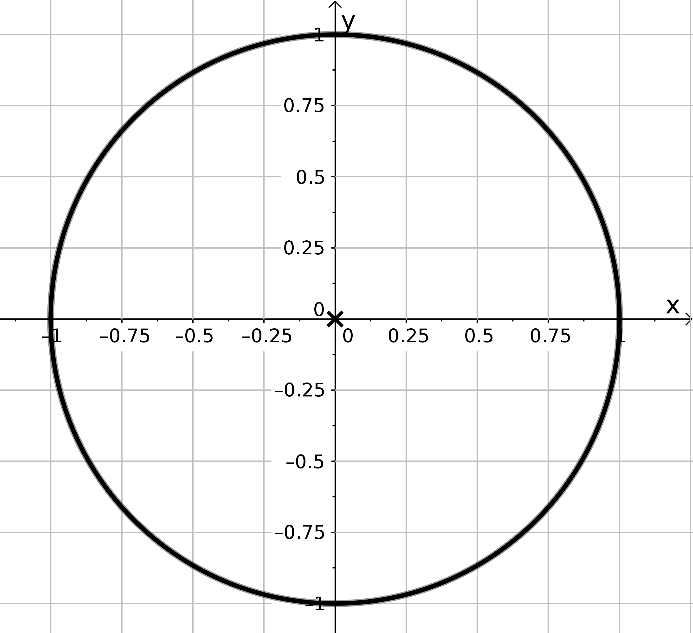
\includegraphics[width=\textwidth]{\trigonometrie/pics/Einheitskreis.png}
	\end{minipage}}%
	\adjustbox{valign=t}{\begin{minipage}{.743\textwidth}
		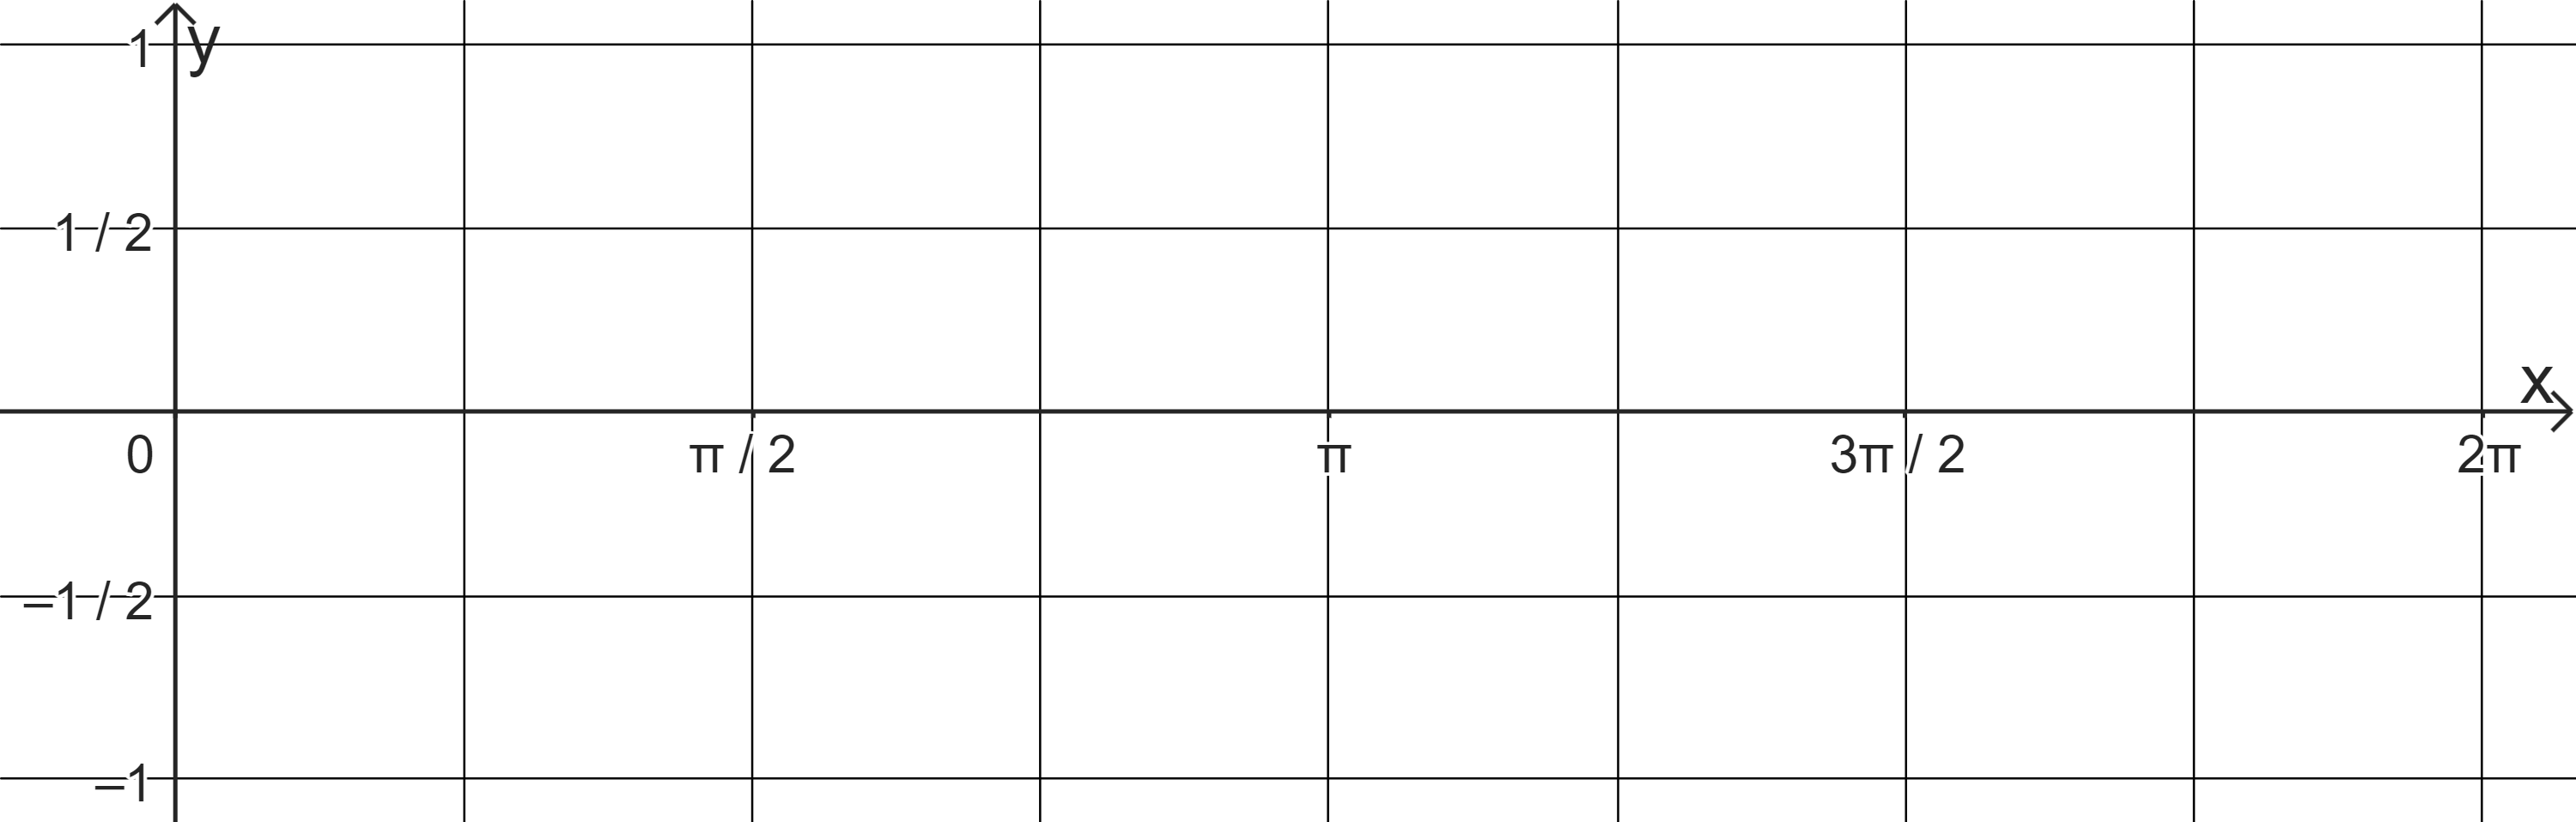
\includegraphics[width=\textwidth]{\trigonometrie/pics/leeresKoordinatensystem.png}
	\end{minipage}}%
\end{minipage}\

\begin{tcolorbox}
	\textbf{Definition der Cosinusfunktion}

	\textcolor{loestc}{Zu jedem Winkel \(b\) kann man genau einen Punkt \(P(x\vert y)\) auf dem Einheitskreis zuordnen. Der Cosinus von \(b\) ist dann die \(x\)-Koordinate dieses Punkts:
		\[\cos\left(b\right)=x\]
	}
\end{tcolorbox}

\textbf{Periode:}

\textcolor{loes}{Die Sinus- und Cosinusfunktion sind beide periodische Funktionen, d.h. sie wiederholen sich nach einer bestimmten Länge unendlich oft. Nach einer Umdrehung auf dem Einheitskreis beginnen beide Funktionen wieder von vorne. Durch Rückwärtsdrehen kann man die beiden Funktionen auch für negative Windel definieren. Die kleinstmögliche Länge auf der \(x\)-Achse, nach der sich eine periodische Funktion wiederholt, wird als Periode \(p\) der Funktion bezeichnet. Für \(\sin x\) und \(\cos x\) ist die Periode jeweils \(p=2\pi\).}